\section{SQL Stored procedures}
\phantomsection

A stored procedure in SQL Server is a group of one or more Transact-SQL statements or a reference to a Microsoft .NET Framework common runtime language (CLR) method. Procedures resemble constructs in other programming languages because they can:
\begin{itemize}
  \item[$\bullet$] Accept input parameters and return multiple values in the form of output parameters to the calling program.
  \item[$\bullet$] Contain programming statements that perform operations in the database. These include calling other procedures.
  \item[$\bullet$] Return a status value to a calling program to indicate success or failure (and the reason for failure).
\end{itemize}
\subsection{Types of Stored Procedures}
There are several types of Stored procedures in SQL Server: \\
\textbf{User-defined}\\
A user-defined procedure can be created in a user-defined database or in all system databases except the Resource database. The procedure can be developed in either Transact-SQL or as a reference to a Microsoft .NET Framework common runtime language (CLR) method.\\
\textbf{Temporary}\\
Temporary procedures are a form of user-defined procedures. The temporary procedures are like a permanent procedure, except temporary procedures are stored in tempdb. There are two types of temporary procedures: local and global. They differ from each other in their names, their visibility, and their availability. Local temporary procedures have a single number sign (\#) as the first character of their names; they are visible only to the current user connection, and they are deleted when the connection is closed. Global temporary procedures have two number signs  as the first two characters of their names; they are visible to any user after they are created, and they are deleted at the end of the last session using the procedure.\\
\textbf{System}\\
System procedures are included with SQL Server. They are physically stored in the internal, hidden Resource database and logically appear in the sys schema of every system- and user-defined database. In addition, the msdb database also contains system stored procedures in the dbo schema that are used for scheduling alerts and jobs.\\
\textbf{Extended User-Defined}\\
Extended procedures enable creating external routines in a programming language such as C. These procedures are DLLs that an instance of SQL Server can dynamically load and run.

\subsection{Benefits of Using the Stored Procedure}

\begin{enumerate}
\item One of the main benefits of using the Stored procedure is that it reduces the amount of information sent to the database server. It can become a more important benefit when the bandwidth of the network is less. Since if we send the SQL query (statement) which is executing in a loop to the server through network and the network gets disconnected, then the execution of the SQL statement doesn't return the expected results, if the SQL query is not used between Transaction statement and rollback statement is not used.
\item Compilation step is required only once when the stored procedure is created. Then after it does not require recompilation before executing unless it is modified and reutilizes the same execution plan whereas the SQL statements need to be compiled every time whenever it is sent for execution even if we send the same SQL statement every time.
\item It helps in re usability of the SQL code because it can be used by multiple users and by multiple clients since we need to just call the stored procedure instead of writing the same SQL statement every time. It helps in reducing the development time.
\item Stored procedure is helpful in enhancing the security since we can grant permission to the user for executing the Stored procedure instead of giving permission on the tables used in the Stored procedure.
\item Sometimes, it is useful to use the database for storing the business logic in the form of stored procedure since it makes it secure and if any change is needed in the business logic, then we may only need to make changes in the stored procedure and not in the files contained on the web server.
\end{enumerate}

\subsection{How to Create a Stored Procedure in SQL Server}
We need to give the procedure a unique name within the schema and then write the sequence of SQL statements to be executed within the procedure. Following is the basic syntax for creating stored procedures:
\lstinputlisting[style=mystyle, language=SQL, caption={Template of a procedure, \cite{doc}}, label=list41,]{sourcecode/tsqlexample.sql}

This template contains parameters for parameter names, procedure name, author name, create date, and so on. These template parameters are in the format <parameter, type, value>:
PARAMETER\_NAME: It is the name of the template parameter in the script.
DATA\_TYPE: It is the optional data type of the template parameter.
VALUE: It is the default value to be used to replace every occurrence of the template parameter in the script.
SET NOCOUNT ON:

1) It gives performance. When SET NOCOUNT is ON, the count (indicating the number of rows affected by a Transact-SQL statement) is not returned. 
2) When SET NOCOUNT is OFF, the count is returned. It eliminates the sending of ONE\_IN\_PROC messages to the client for each statement in a stored procedure. 
3) For stored procedures that contain several statements that do not return much actual data, this can provide a significant performance boost because network traffic is greatly reduced. The setting of SET NOCOUNT is set at execute or run time and not at parse time.
 
RETURN:

1) Return values indicate a return code from the stored procedure. The return value does not have to be specified as the parameters do. We simply use the RETURN SQL statement to return a value. This value has to be an Integer data type and can return any value you need. For example, this value can be a return code, the number of rows affected by a SQL statement, or the number of rows in a table. Basically any integer data that you want to return can be specified in a return value in your stored procedure.

2) The RETURN statement exits unconditionally from a stored procedure, so the statements following RETURN are not executed. Though the RETURN statement is generally used for error checking, you can use this statement to return an integer value for any other reason. Using RETURN statement can boost performance because SQL Server will not create a recordset.

% \lstinputlisting[style=mystyle, language=SQL, caption={Caption of the listing code, \cite{doc}}, label=list41,]{sourcecode/minmax.sql}

% \begin{figure}[ht!]
%     \centering
%     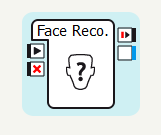
\includegraphics[width=0.2\textwidth]{face_reco}
%     \caption{}
%     \label{fig_21}
% \end{figure}

\clearpage